\section{Introduction}

\begin{figure}[t]
\centering
\includegraphics[width=0.45\textwidth]{figures/taxonomylabels}
 \caption{A toy example of taxonomy}
\label{fig:taxonomyexample}
\end{figure}


\begin{figure}[t]
\centering
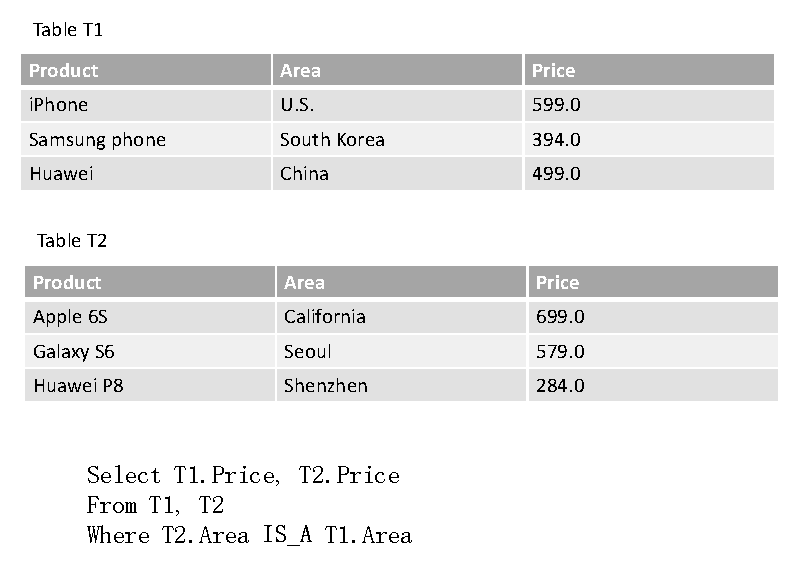
\includegraphics[width=0.45\textwidth]{figures/productexample}
 \caption{Examples to illustrate approximate joins}
\label{fig:twotables}
\end{figure}



 String joins, which find all string pairs between two input string collections, are essential operations in many applications, such as  data integration \cite{conf/sigmod/Sarawagi04}, data cleansing \cite{conf/vldb/ArasuGK06,journals/www/LiJM06} and record linkage \cite{books/Winkler99}. Conceptually, there are two cases of string joins: \textit{exact-joins} and \textit{approximate-joins}. Exact joins mean that two matching strings are exactly the same, while approximate joins tolerate certain difference between two strings and the similarity of two strings is measured by a similarity function, such as  Levenshtein Distance
\cite{journals/pvldb/XiaoWL08,conf/sigmod/WangLF12},  Jaccard
similarity~\cite{conf/icde/ChaudhuriGK06} and cosine
similarity~\cite{journals/ipm/SaltonB88}.

Recently, there are some work to improve the effectiveness of string joins by using synonym. Their observation is that the exisitng similarity function can only capture the syntatic similarity, but not semantic. Two string may present the same entity, but their spelling are completely. differently. For a given word, we can use WordNet [4] to find its synonyms
or find terms that have concept-instance relationships
with the word. These are good candidates for string joins. But WordNet does not contain information such as
Microsoft is an IT company, or Kindle is a popular e-Reader.
Still, terms such as IT company, Kindle, Microsoft are frequently
used in data sets. Some recent work (e.g., [26, 21])
focuses on automatically discovering relationships among
terms by mining web pages and search engine click logs.
This enables us to find important concept-instance relationship
for large sets of terms.
 Taxonomies are sets of IS-A hierarchies, which identify the relations between different concepts.

In this paper, we assume that we already have complete
information of term substitutions, and we will focus on how
to efficiently perform a string join by utilizing the taxonomy, and how to optimize the index structure
for this purpose.

For example, Figure \ref{fig:taxonomyexample} shows an example of a taxonomy tree for geographical concepts.   In general, the taxonomy presents a general-purpose strategy to improve the accuracy of string joins by enriching data with semantics-based knowledge  (i.e., a set of IS-A hierarchies). For example, Figure \ref{fig:twotables} shows two tables  from different sources about produce information. If we perform a traditional string join based on area, then there is no any matching results. But based on the taxonomy, if we know that California is a state of U.S. and Apple 6s is a model of Iphone. Then the first records of two tables are possible matching records.

The concept-instance
relationship defines a taxonomy. The substitution relationship
is a transitive closure of the concept-instance relationship.
For example, if ``puppy'' is an instance of ``dog'', and
``dog'' is an instance of ``pet'', then ``puppy'' could be a substitute
of ``pet''. If we treat each term as a node, and create
for each (concept, instance) pair, an edge from the concept
to the instance, then we can think of the taxonomy as a directed tree or forest. For any node that representing a term,
its substitute could be any descendant of it in the tree. Figure
1 gives an example of a concept-instance taxonomy.


For the exact-join with taxonomy, we can extend the above SQL language to support. For example,
consider the following SQL script:

\vspace{2mm}

\noindent \textsf{Select T1.price, T2.price} \\
\noindent \textsf{ From T1 and T2} \\
\noindent   \textsf{Where T2.product \textbf{IS-A} T1.product and T2.area \textbf{IS-A} T1.area}

 \vspace{2mm}


\noindent which shows a very simple SQL script that
perform the join between two tables in Figure \ref{fig:twotables}.
In the figure, the area and product name are performed the IS-A relations. This script the ``IS-A'' predicate.


For the approximate joins, the brute-force algorithm that enumerates every string pair and checks whether the two strings in the pair are similar is rather expensive. To alleviate this problem, many algorithms have been proposed in the recent two decades. One widely-adopted technique employs a filter-verification framework, which includes two steps: (1) Filter step: devising effective filtering algorithms to prune large numbers of dissimilar pairs and generating a set of candidate pairs; and (2) Verification step: verifying each candidate pair by computing
the real similarity and outputting the final results. Filtering algorithms in the first step play an important role
in the framework. Most of existing filtering algorithms employ a signature-based technique, which generates signatures for each string such that if two strings are similar, their signatures must have overlaps. Thus the signature-based technique can prune string pairs that have no common signature.

Recently many filtering techniques have been proposed, e.g., count filtering [8,13,18], length filtering [8,14], position
filtering [25,27], prefix filtering [4] and content filtering [25]. As prefix filtering is the most effective filtering technique,
many algorithms have been proposed to optimize prefix filtering for different similarity metrics, e.g., AllPair [2],
PPJoin [27], EDJoin [25], QChunk [17], VChunk [24], AdaptJoin [23]. There are also many other signature schemes, e.g., PartEnum [1],
PassJoin [14], FastSS [20].

Unfortunately, these algorithms are not easily extended to process taxonomy. Because all the existing methods are based on the observation that two strings are similar only if their signatures overlap. But this is not true for taxonomy, because two strings may have IS-A relation without any common tokens (signatures).

The leave behind two intriguing questions:

1. How to efficient process string joins with taxonomy? And for multiple joins.


2. How to process the similarity joins and multiple-way similarity joins?  This question becomes increasingly urgent nowadays with the arrival of big data.

When we tried to apply these known technologies in our taxonomy environment, however, we encounter a few critical challenges, summarized as below:

\noindent \textit{Taxonomy signature}

\noindent \textit{Taxonomy update}

%\begin{problem}(String measure with taxonomy). Given two strings $s_1$ and $s_2$ and a taxonomy $T$, how to measure the similarity between $s_1$ and $s_2$ based on T?
%\end{problem}
%\begin{problem}(String joins with taxonomy). Given a string $p$$\in$
%$\Sigma^*$, an integer k, and a synonym set $\mathbb{R}$,  .
%\end{problem}




\subsection{Novelty and contributions}


\smallskip


Our contributions are as follows.

\noindent \textbf{Introduction of string joins with taxonomy}. We introduce a new problem to utilize the taxonomy for the string joins in databases, which has application in data integration and data cleansing.

\noindent \textbf{Optimal algorithms for string joins} We introduce a holistic algorithm for multiple string joins.

\noindent \textbf{Introduction of approximate string joins with taxonomy}: Provide three relationships Hyper, Hypo and mixed similarity.

\noindent \textbf{Novel algorithms for approximate string joins}

\noindent \textbf{Novel algorithms for taxonomy update}  We introduce a novel algorithm for incrementally updating taxonomy. Our merging algorithm allows us to incorporate new correlations introduced over a subset of tuples into
the correlations already present in the database, without recomputing the existing results.


Finally, we perform experiments to evaluate our results and show the benefits of proposal algorithms.


\smallskip

The rest of this paper is organized as follows. Section 2
provides the necessary definitions, formulates . Section
3 includes our algorithm for exact joins with taxonomy. In Section 4, we study
the approximate string join, proposing our solution, analyzing its approximation
ratio, and presenting our similarity join algorithms.
Our experiments are presented in Section 5. Finally,
Section 6 concludes with a discussion about future work.
